\section{Análise descritiva dos lobistas}
\label{sec:resultados_descritica_lobistas}
Avaliação da distribuição dos lobistas registados junto às instituições europeias.

\begin{table}[!htbp]
\centering
\caption{Distribuição de organizações por categoria}
\begin{tabular}{lrr}
\toprule
Categoria & Total & (\%) \\
\midrule
Empresas & 5770 & 46.300 \\
ONGs & 3480 & 27.900 \\
Outros & 3218 & 25.800 \\
\bottomrule
\end{tabular}

\end{table}

A Tabela acima apresenta a composição do universo de lobistas por categoria organizacional. Observa-se o predomínio de entidades empresariais e organizações da sociedade civil. A categoria \textit{Outros} abrange uma variedade de organizações, incluindo representações governamentais, universidades, sindicatos, associações profissionais, \textit{think tanks}, consultorias profissionais, instituições acadêmicas, redes de autoridades públicas, organizações religiosas, escritórios de advocacia e entidades estabelecidas por países terceiros, conforme a classificação detalhada no registro de transparência.

O resultado reforça assimetrias moderadas entre categorias e não sugere concentração extrema em um único tipo organizacional. Em termos substantivos, isso indica competição horizontal por acesso e agenda entre perfis empresariais e societais.

% \paragraph{País-sede e ano de registo}
% \begin{table}[!htbp]
% \centering
% \caption{Distribuição de lobistas por país-sede}
% \begin{tabular}{lrrr}
\toprule
País-sede & Total & (\%) & Membro da UE \\
\midrule
BELGIUM & 2270 & 18.200 & True \\
GERMANY & 1740 & 14.000 & True \\
FRANCE & 1165 & 9.300 & True \\
UNITED KINGDOM & 787 & 6.300 & False \\
NETHERLANDS & 786 & 6.300 & True \\
SPAIN & 780 & 6.300 & True \\
ITALY & 753 & 6.000 & True \\
UNITED STATES & 567 & 4.500 & False \\
AUSTRIA & 312 & 2.500 & True \\
FINLAND & 297 & 2.400 & True \\
SWEDEN & 293 & 2.400 & True \\
SWITZERLAND & 276 & 2.200 & False \\
POLAND & 251 & 2.000 & True \\
DENMARK & 224 & 1.800 & True \\
IRELAND & 209 & 1.700 & True \\
PORTUGAL & 177 & 1.400 & True \\
GREECE & 154 & 1.200 & True \\
CZECH REPUBLIC & 139 & 1.100 & False \\
ROMANIA & 120 & 1.000 & True \\
NORWAY & 105 & 0.800 & False \\
HUNGARY & 91 & 0.700 & True \\
LUXEMBOURG & 83 & 0.700 & True \\
ESTONIA & 67 & 0.500 & True \\
CROATIA & 66 & 0.500 & True \\
LITHUANIA & 62 & 0.500 & True \\
SLOVENIA & 57 & 0.500 & True \\
SLOVAKIA & 54 & 0.400 & True \\
BULGARIA & 52 & 0.400 & True \\
CANADA & 46 & 0.400 & False \\
MALTA & 42 & 0.300 & True \\
LATVIA & 31 & 0.200 & True \\
UKRAINE & 29 & 0.200 & False \\
JAPAN & 26 & 0.200 & False \\
CYPRUS & 24 & 0.200 & True \\
BRAZIL & 23 & 0.200 & False \\
AUSTRALIA & 20 & 0.200 & False \\
TURKEY & 20 & 0.200 & False \\
ISRAEL & 19 & 0.200 & False \\
SERBIA & 19 & 0.200 & False \\
ALBANIA & 11 & 0.100 & False \\
SINGAPORE & 10 & 0.100 & False \\
UNITED ARAB EMIRATES & 10 & 0.100 & False \\
NEW ZEALAND & 8 & 0.100 & False \\
CHINA & 8 & 0.100 & False \\
INDIA & 8 & 0.100 & False \\
MOROCCO & 7 & 0.100 & False \\
SOUTH AFRICA & 7 & 0.100 & False \\
SENEGAL & 6 & 0.000 & False \\
MALAYSIA & 6 & 0.000 & False \\
MEXICO & 6 & 0.000 & False \\
NIGERIA & 6 & 0.000 & False \\
BOSNIA-HERZEGOVINA & 6 & 0.000 & False \\
LIECHTENSTEIN & 5 & 0.000 & False \\
MOLDOVA, REPUBLIC OF & 5 & 0.000 & False \\
THAILAND & 5 & 0.000 & False \\
KOREA, REPUBLIC OF & 5 & 0.000 & False \\
TAIWAN & 4 & 0.000 & False \\
LEBANON & 4 & 0.000 & False \\
ECUADOR & 4 & 0.000 & False \\
COLOMBIA & 4 & 0.000 & False \\
ICELAND & 3 & 0.000 & False \\
PALESTINIAN OCCUPIED TERRITORY & 3 & 0.000 & False \\
INDONESIA & 3 & 0.000 & False \\
KENYA & 3 & 0.000 & False \\
BERMUDA & 3 & 0.000 & False \\
JORDAN & 3 & 0.000 & False \\
GEORGIA & 3 & 0.000 & False \\
ARGENTINA & 3 & 0.000 & False \\
HONG KONG & 3 & 0.000 & False \\
RUSSIA, FEDERATION OF & 3 & 0.000 & False \\
GHANA & 3 & 0.000 & False \\
MONACO & 3 & 0.000 & False \\
ZAMBIA & 2 & 0.000 & False \\
NIGER & 2 & 0.000 & False \\
MONTENEGRO & 2 & 0.000 & False \\
KAZAKHSTAN & 2 & 0.000 & False \\
PHILIPPINES & 2 & 0.000 & False \\
COSTA RICA & 2 & 0.000 & False \\
DOMINIQUE & 2 & 0.000 & False \\
URUGUAY & 2 & 0.000 & False \\
ARMENIA & 2 & 0.000 & False \\
TUNISIA & 2 & 0.000 & False \\
VENEZUELA & 2 & 0.000 & False \\
NORTH MACEDONIA & 2 & 0.000 & False \\
MAURITANIA & 1 & 0.000 & False \\
REUNION & 1 & 0.000 & False \\
GIBRALTAR & 1 & 0.000 & False \\
CONGO, DEMOCRATIC REPUBLIC OF & 1 & 0.000 & False \\
QATAR & 1 & 0.000 & False \\
DOMINICAN REPUBLIC & 1 & 0.000 & False \\
CHILE & 1 & 0.000 & False \\
SRI LANKA & 1 & 0.000 & False \\
BOLIVIA & 1 & 0.000 & False \\
VIETNAM & 1 & 0.000 & False \\
OMAN & 1 & 0.000 & False \\
MACAO & 1 & 0.000 & False \\
MONGOLIA & 1 & 0.000 & False \\
COTE D'IVOIRE & 1 & 0.000 & False \\
ZIMBABWE & 1 & 0.000 & False \\
NAMIBIA & 1 & 0.000 & False \\
NEPAL & 1 & 0.000 & False \\
LAOS, PEOPLE'S DEMOCRATIC REPUBLIC & 1 & 0.000 & False \\
BARBADOS & 1 & 0.000 & False \\
BURKINA FASO & 1 & 0.000 & False \\
KOSOVO & 1 & 0.000 & False \\
PAPUA NEW GUINEA & 1 & 0.000 & False \\
GABON & 1 & 0.000 & False \\
PAKISTAN & 1 & 0.000 & False \\
CAMEROON & 1 & 0.000 & False \\
FAROE ISLANDS & 1 & 0.000 & False \\
GUATEMALA & 1 & 0.000 & False \\
MYANMAR & 1 & 0.000 & False \\
CONGO & 1 & 0.000 & False \\
RUANDA & 1 & 0.000 & False \\
MALI & 1 & 0.000 & False \\
TRINIDAD AND TOBAGO & 1 & 0.000 & False \\
PARAGUAY & 1 & 0.000 & False \\
TOGO & 1 & 0.000 & False \\
CAMBODIA & 1 & 0.000 & False \\
TANZANIA, UNITED RE UBLIC OF & 1 & 0.000 & False \\
UGANDA & 1 & 0.000 & False \\
\bottomrule
\end{tabular}

% \end{table}

A distribuição geográfica evidencia forte concentração em Estados-Membros centrais: Bélgica (18,2\%), Alemanha (14,0\%) e França (9,3\%). Países como Países Baixos, Espanha, Reino Unido e Itália aparecem na sequência (6\% cada). Nota-se presença extracomunitária não desprezível. Cerca de 19\% são de países não membros da \cite{UE} (com destaque para os Estados Unidos, com 4,5\% dos lobistas registrados), sinalizando a atratividade regulatória do mercado europeu.

\begin{figure}[!htbp]
\centering
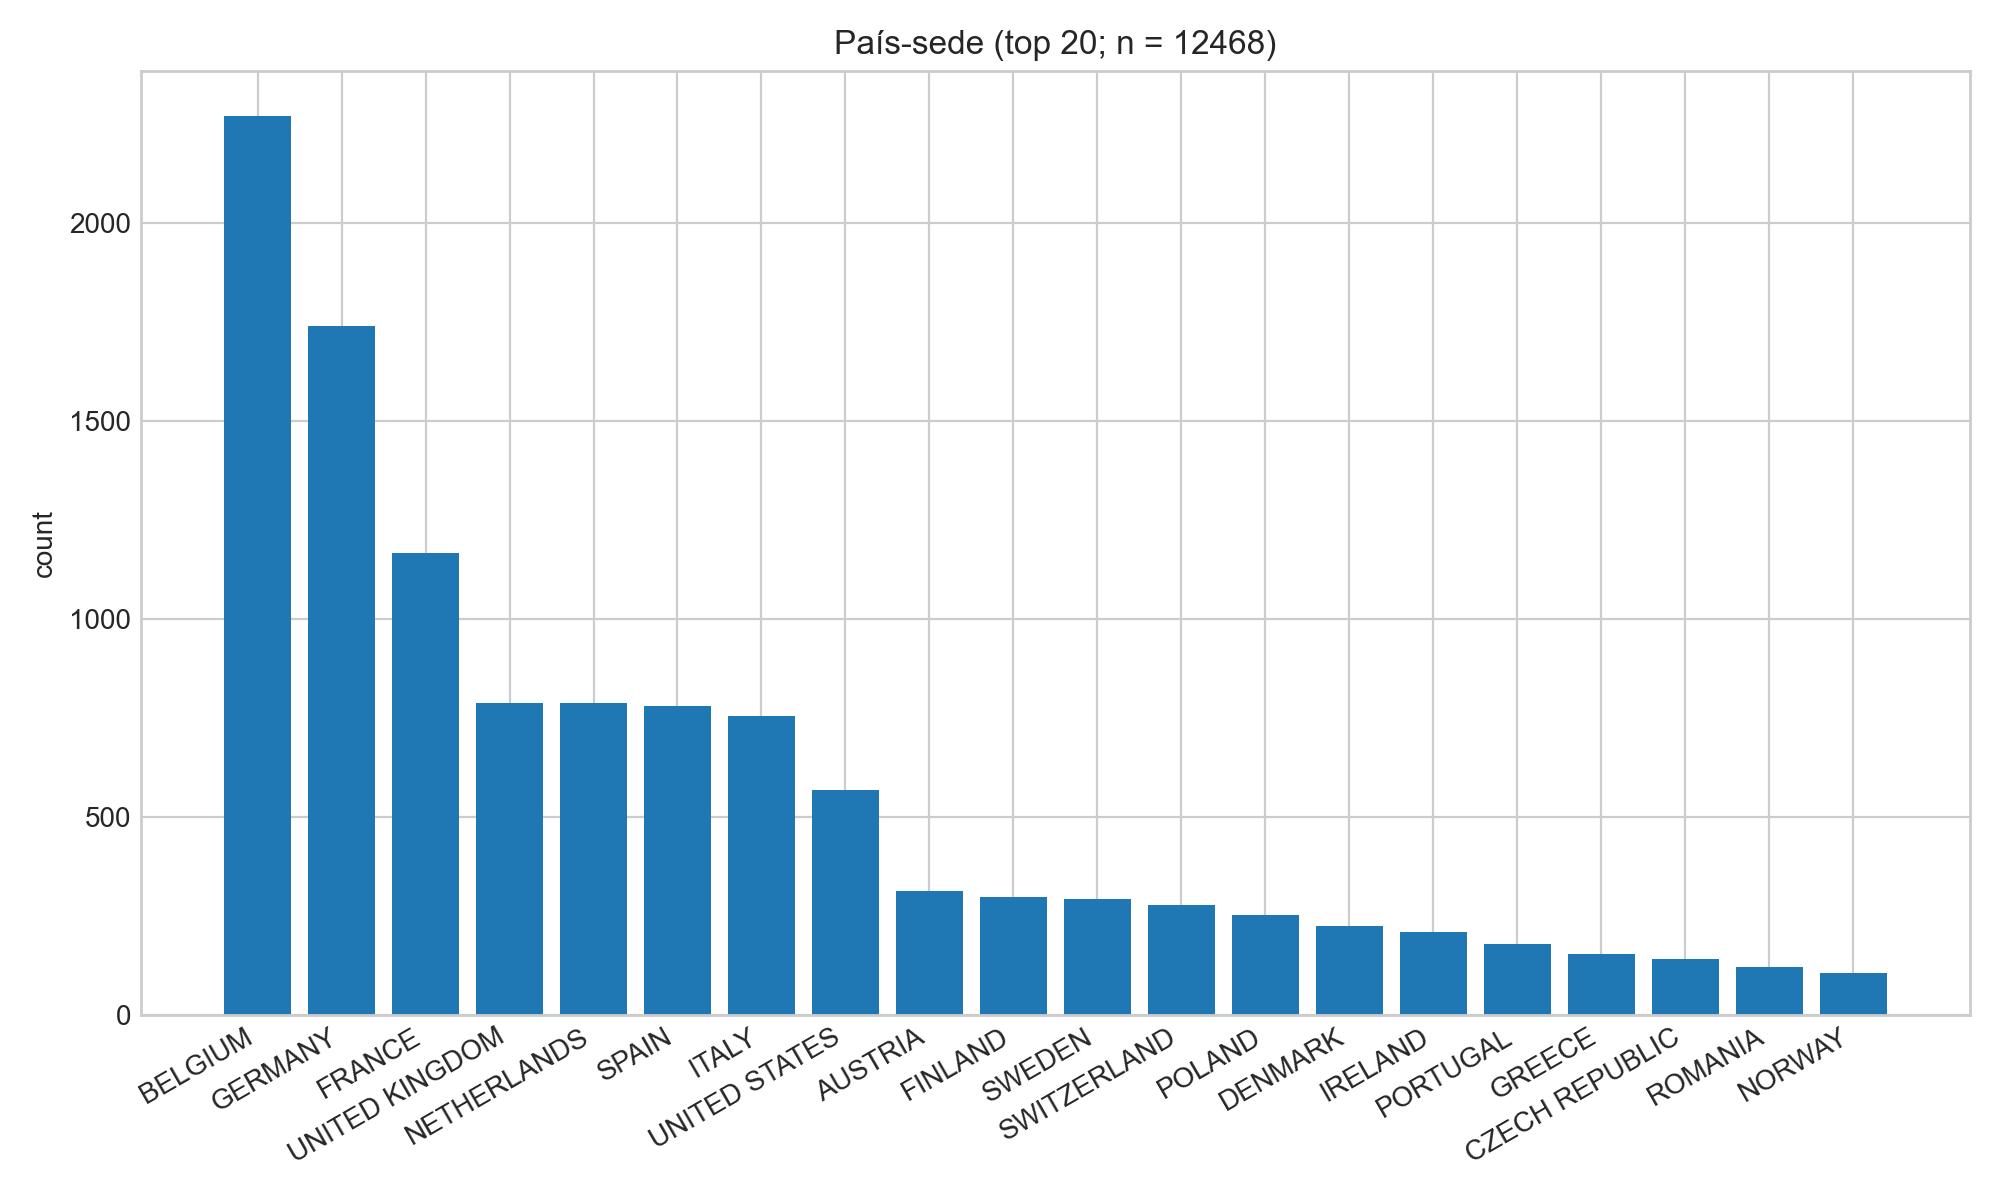
\includegraphics[width=0.9\textwidth]{figures/country_distribution_top20.png}
\caption{Top 20 países-sede (n = 12.468 organizações, totalizando 91\% do total de organizações)}
\end{figure}

O recorte dos \textit{top 20} evidencia uma cauda longa: muitos países com baixas frequências, consistentes com a internacionalização seletiva do \textit{lobbying}. O padrão é coerente com hipóteses de \textit{venue shopping} e vantagens de proximidade institucional em Bruxelas/Strasburgo.

Temporalmente, observa-se aceleração do registro de entidades após meados da década de 2010, com 2023 concentrando 17,9\% do total. Picos intermediários (2015--2016; 2020--2022) são compatíveis com ciclos legislativos, janelas regulatórias e alterações incrementais nos mecanismos de transparência.

\begin{figure}[!htbp]
\centering
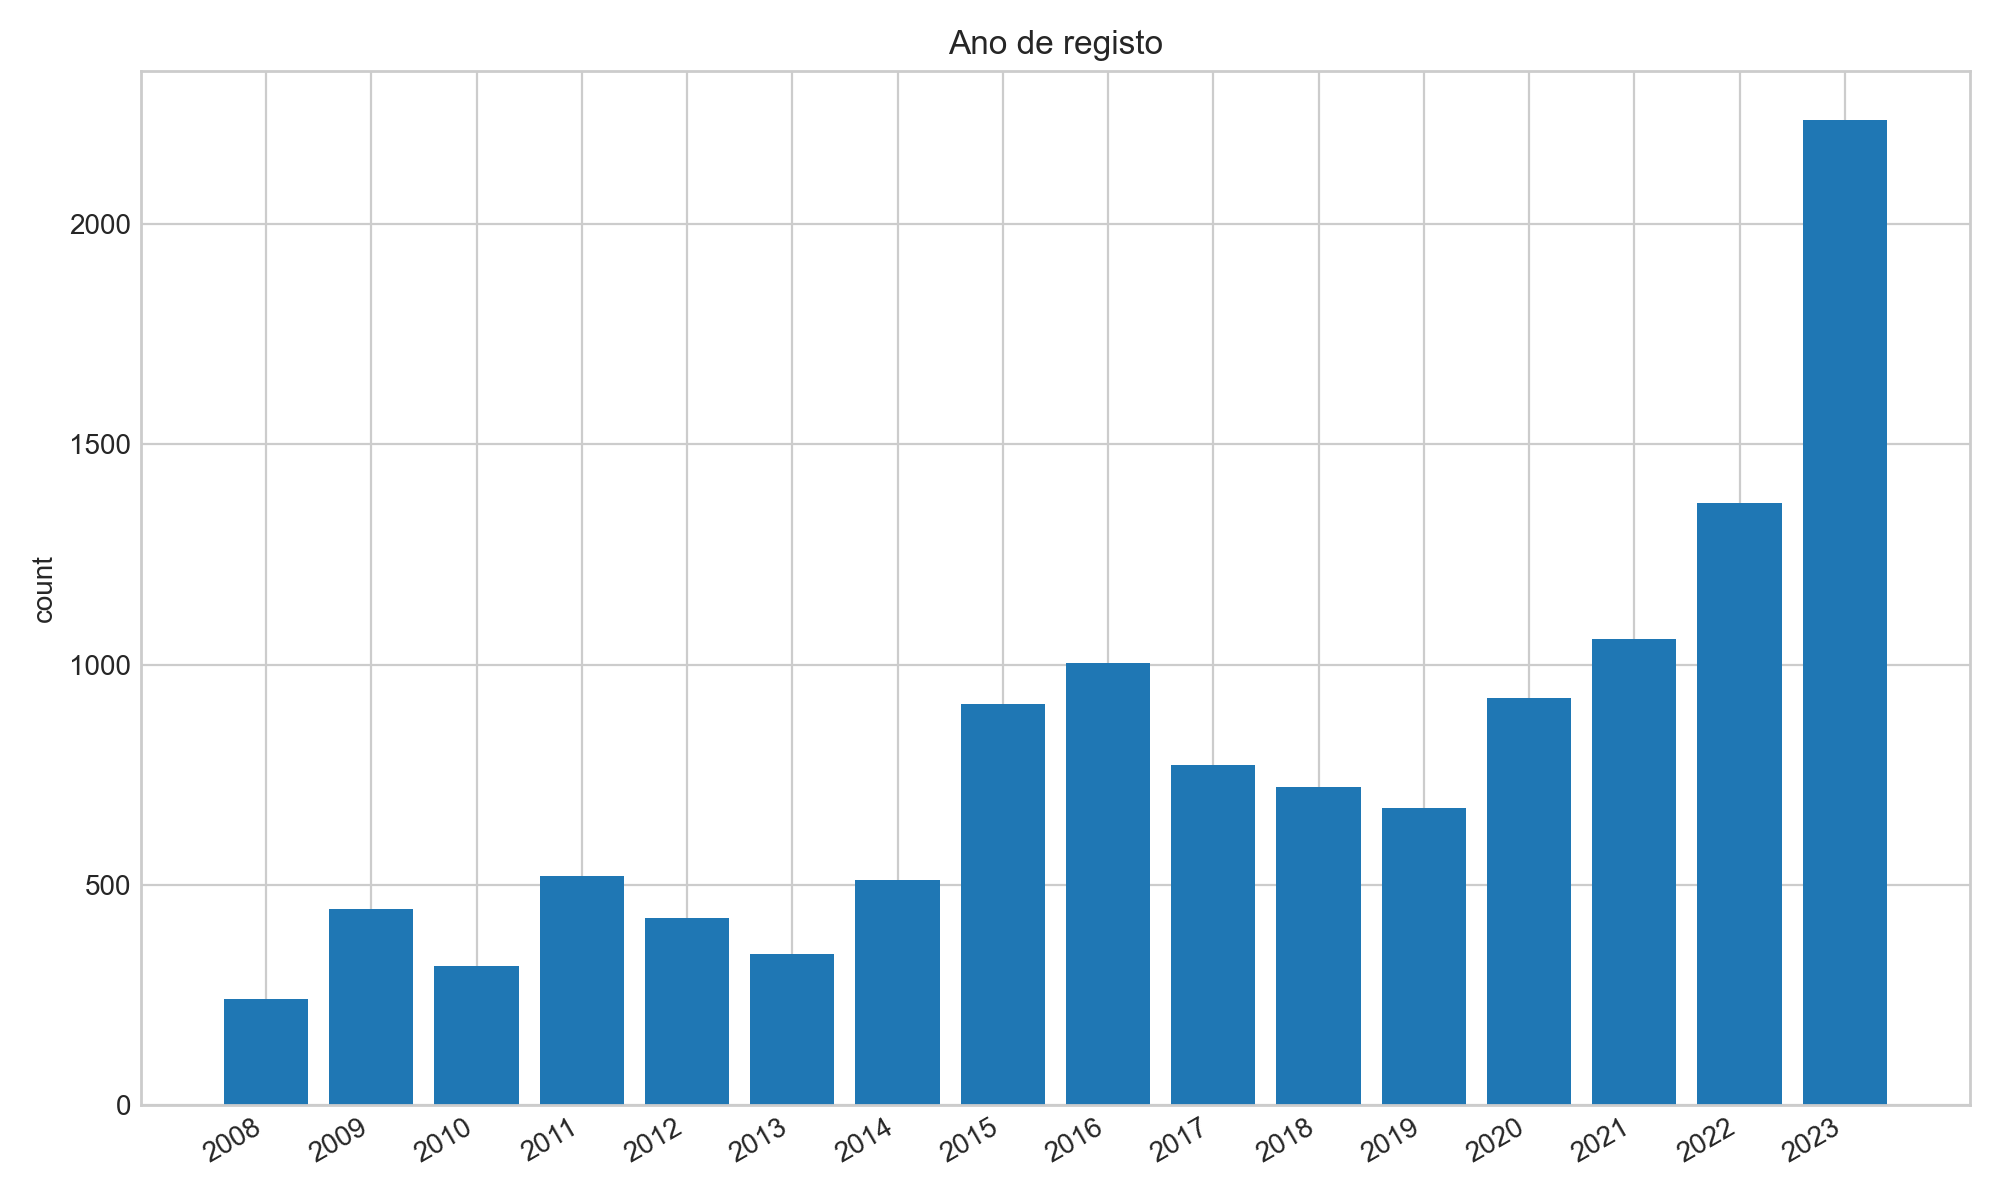
\includegraphics[width=0.75\textwidth]{figures/year_distribution.png}
\caption{Ano de registo}
\end{figure}

O padrão visual sugere crescimento estrutural recente do ecossistema de representação de interesses, possivelmente associado às agendas de transição digital e verde e à recomposição pós-pandemia.

As incidências por domínio destacam \textit{Infraestrutura e Indústria} (68,3\%), \textit{Tecnologia} (67,9\%) e \textit{Economia e Comércio} (67,4\%), seguidas por \textit{Ambiente e Clima} (64,7\%) e \textit{Assuntos Externos e Segurança} (51,3\%). Temas como \textit{Saúde} (43,7\%) e \textit{Educação} (41,2\%) são intermediários; \textit{Agricultura} (35,3\%) e \textit{Direitos Humanos} (25,3\%) têm menor incidência relativa.

\begin{figure}[!htbp]
\centering
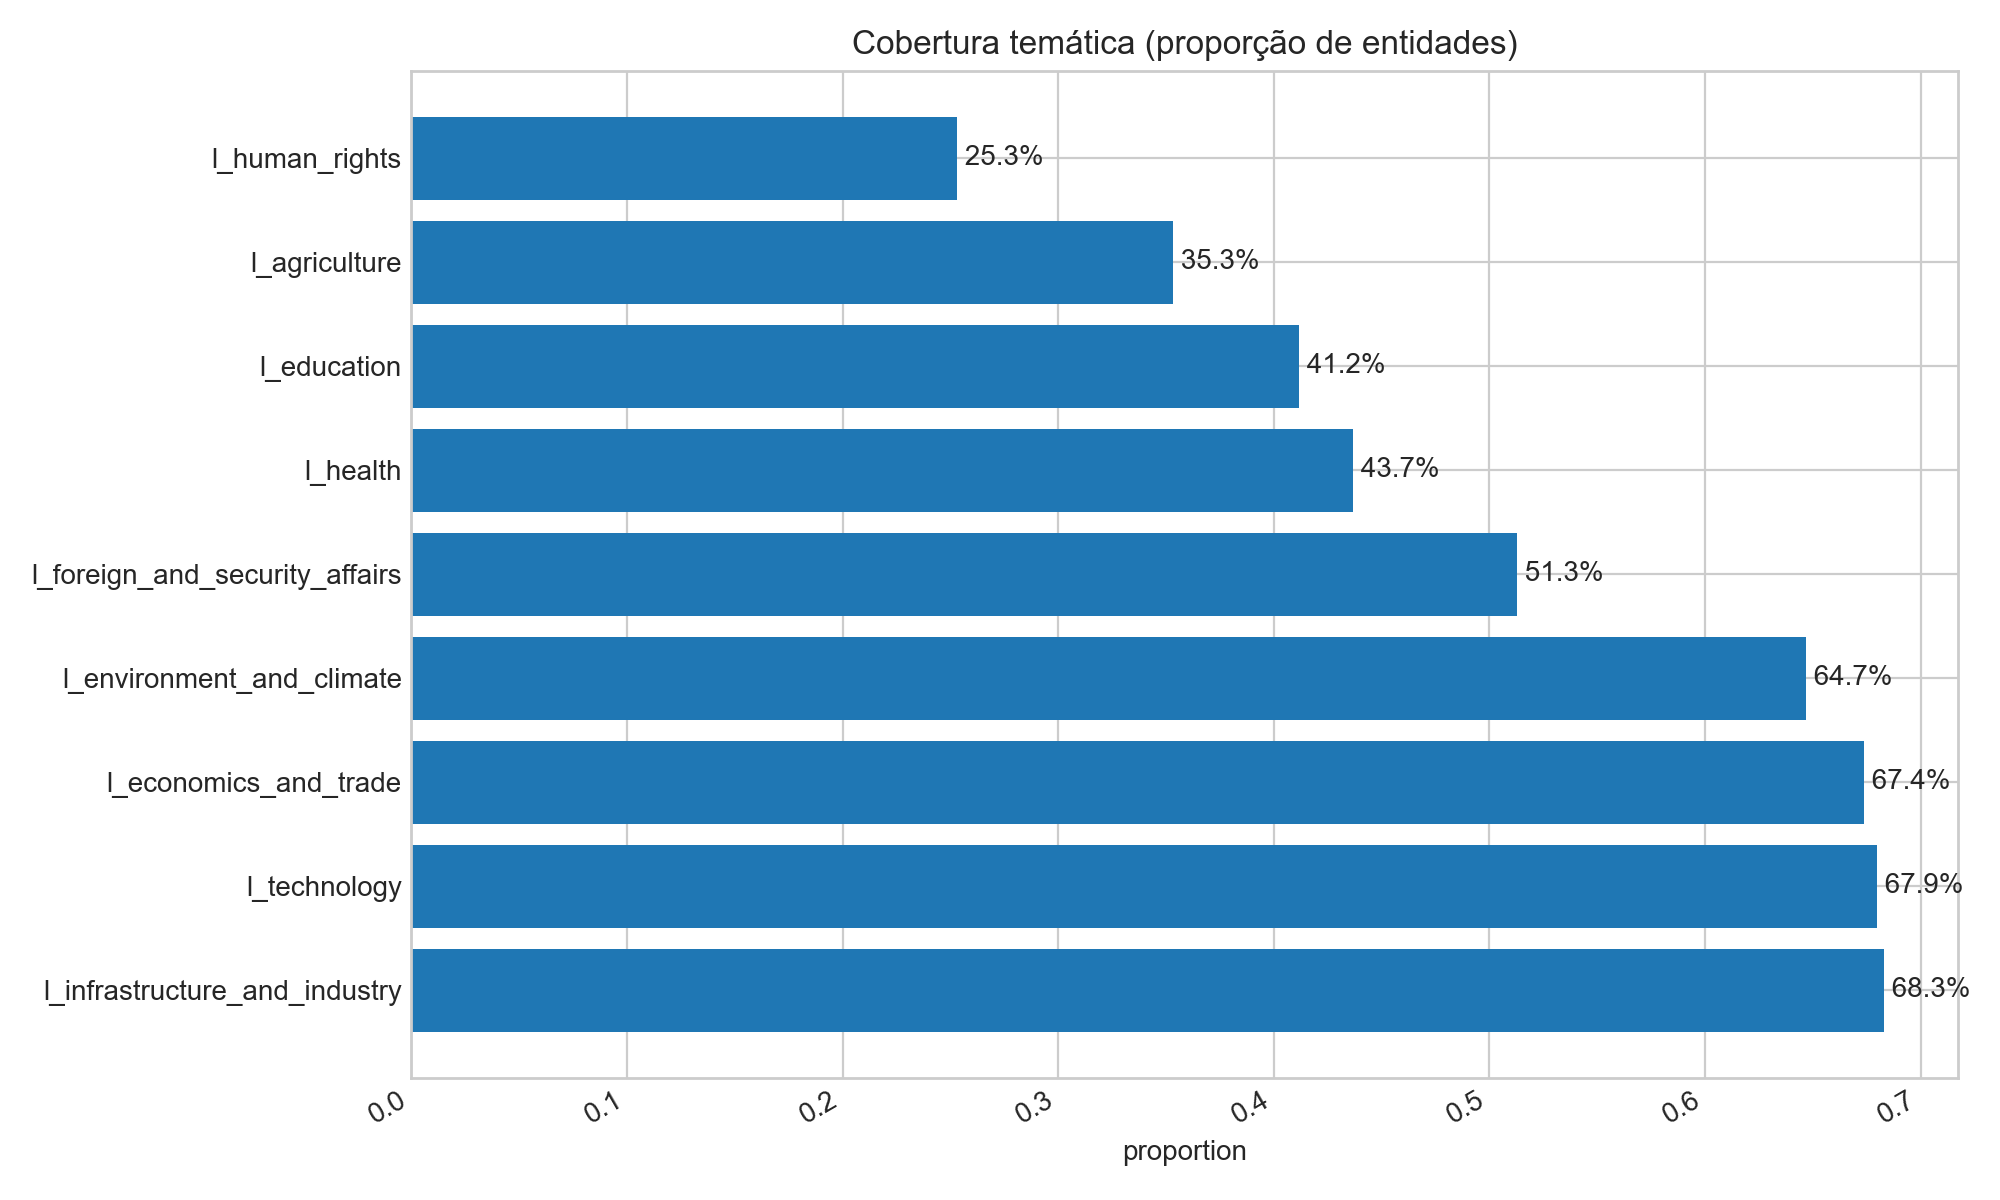
\includegraphics[width=0.9\textwidth]{figures/theme_coverage.png}
\caption{Cobertura temática (proporção de entidades)}
\end{figure}

O ordenamento por proporção sugere centralidade de agendas de competitividade industrial, digitalização e cadeias de valor, bem como a transversalidade da pauta ambiental.


\begin{figure}[!htbp]
\centering
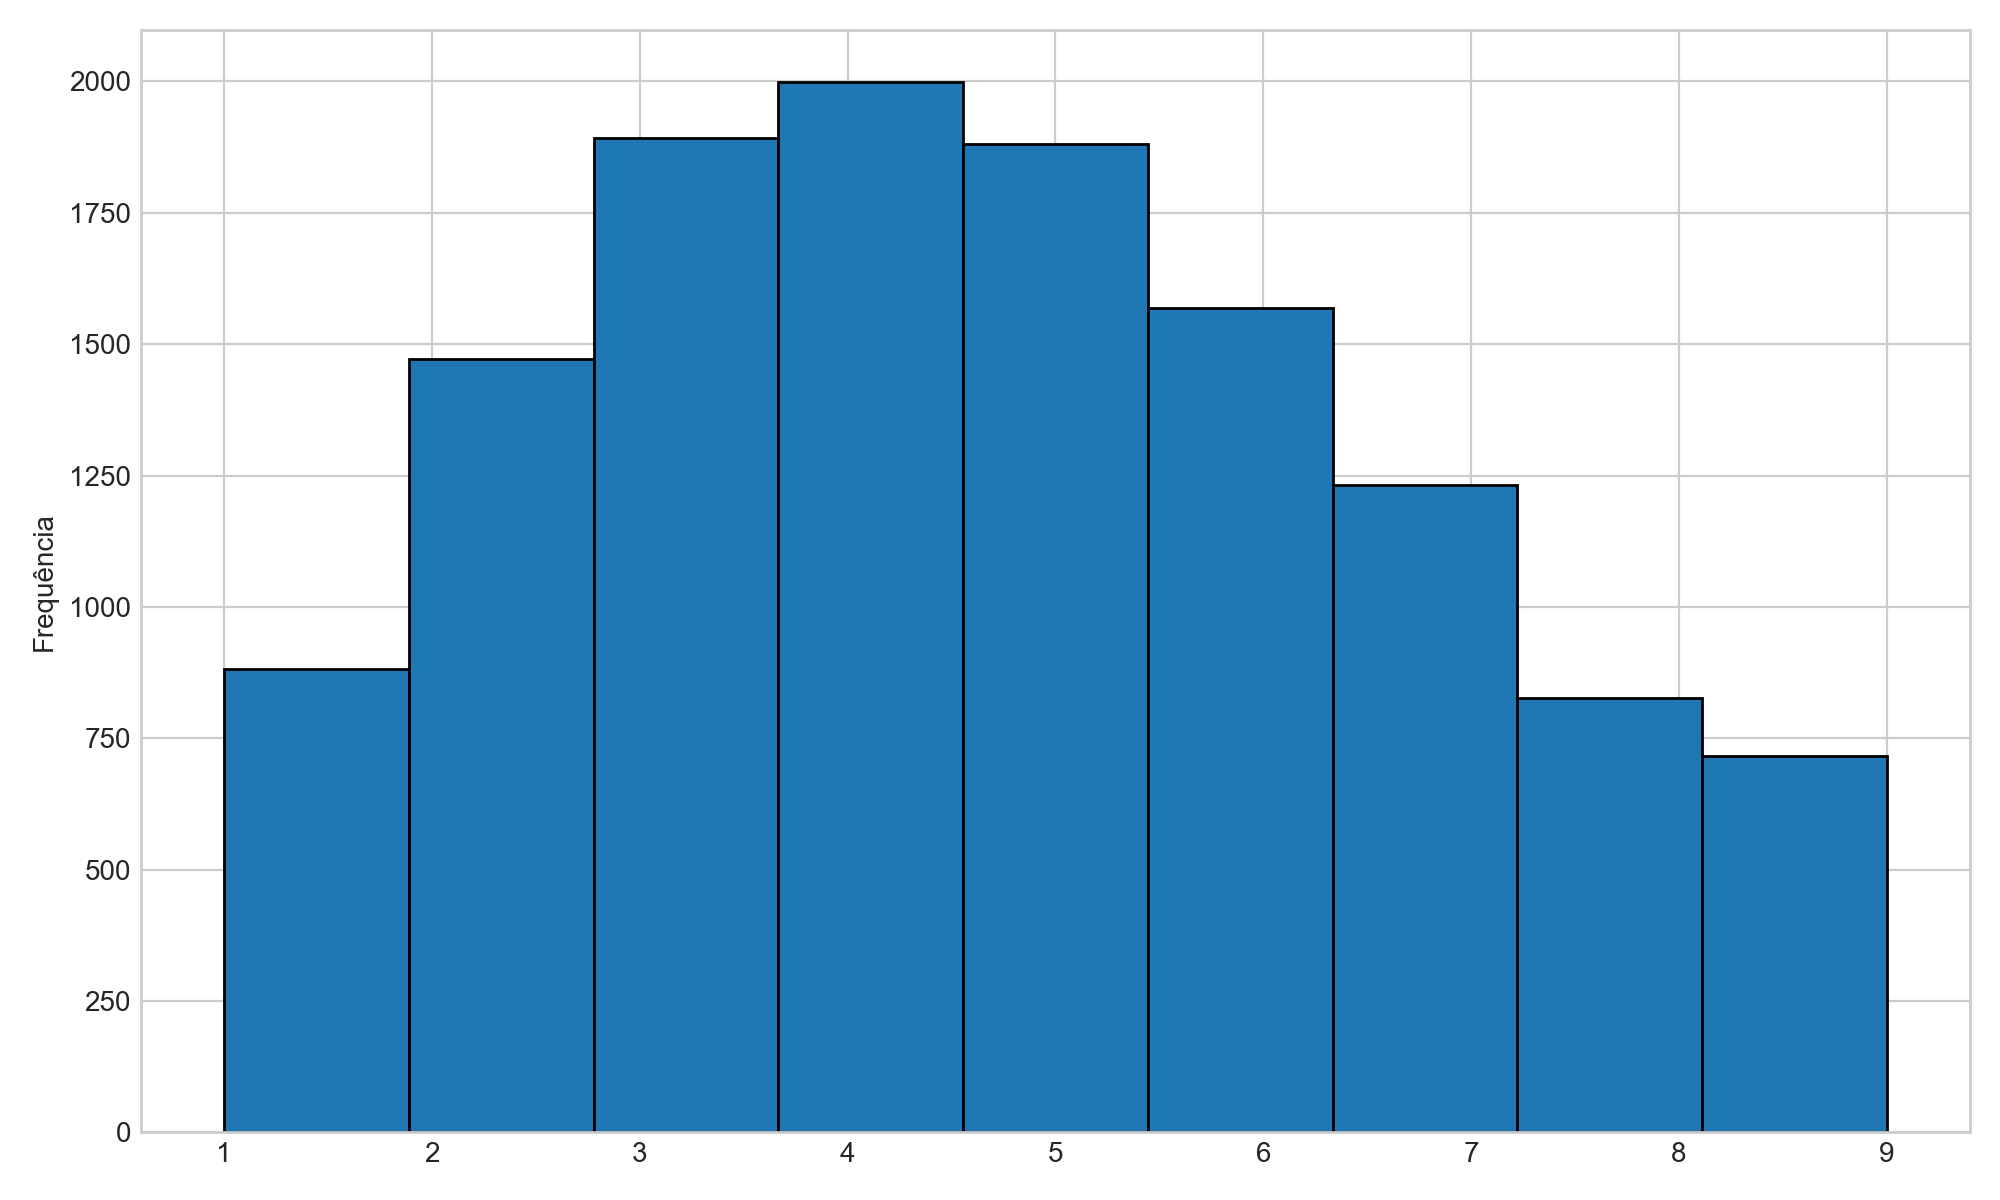
\includegraphics[width=0.75\textwidth]{figures/themes_per_lobbyist_hist.png}
\caption{Número de temas por lobista}
\end{figure}

A distribuição do número de temas por entidade indica a coexistência de atores multi-temáticos e especializados. Esse traço é relevante para a modelagem, pois sugere que a intensidade de esforço (extensivo vs. intensivo) varia com o perfil organizacional e o ambiente regulatório dos domínios.


As estatísticas de orçamento máximo declarado (em escala logarítmica) indicam mediana em torno de 11,5 e quartis aproximadamente entre 10,1 e 12,9. A presença de valores inválidos/extremos na base administrativa (por exemplo, ocorrências infinitas) distorce a média e o desvio-padrão, recomendando foco em medidas robustas (mediana, intervalos interquartílicos) e rotinas de limpeza nos exercícios inferenciais.

\begin{figure}[!htbp]
\centering
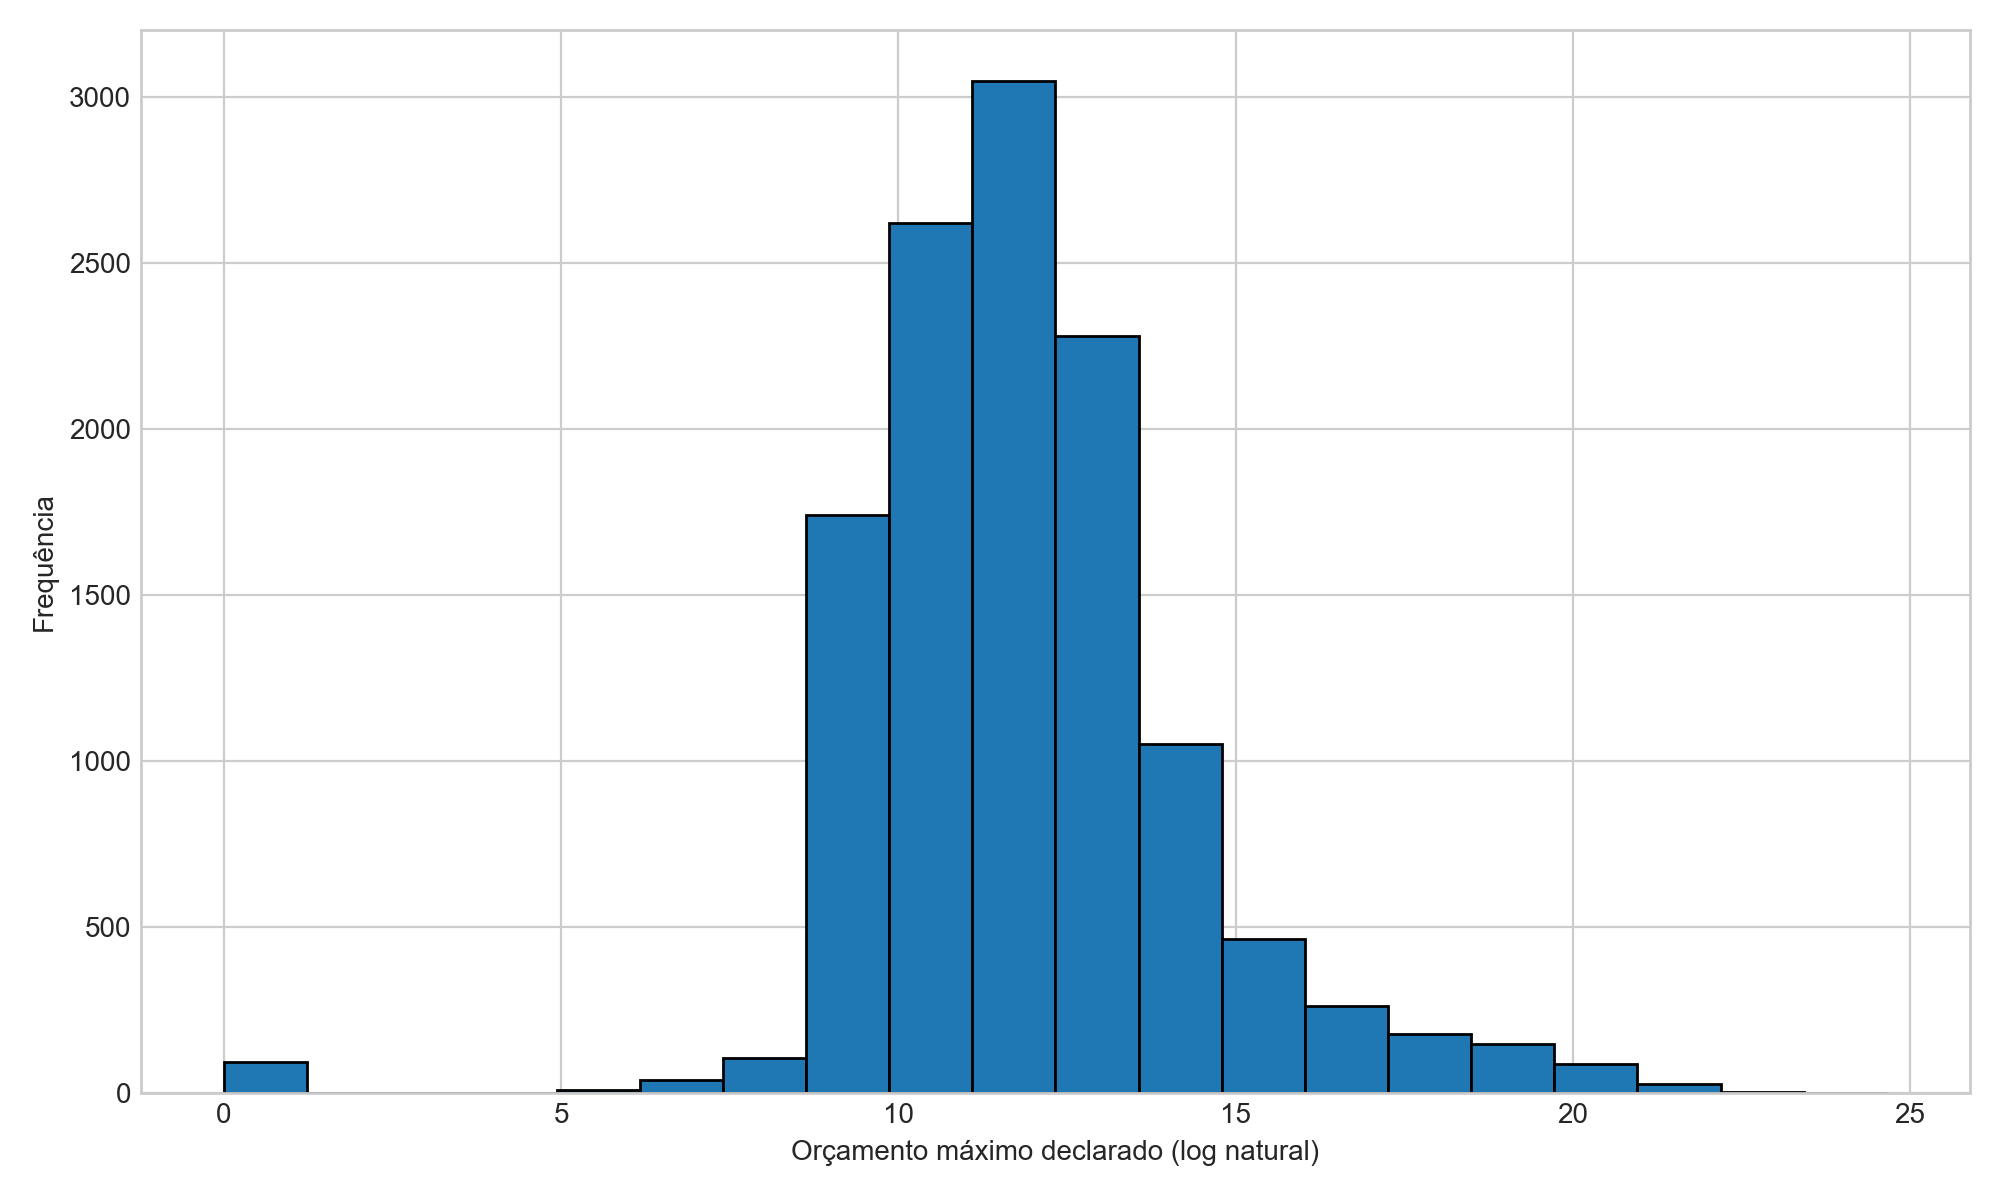
\includegraphics[width=0.75\textwidth]{figures/budget_ln_hist.png}
\caption{Distribuição de orçamento máximo declarado ($ln(budget)$)}
\end{figure}

A distribuição apresenta assimetria e cauda à direita compatíveis com heterogeneidade de porte organizacional, sugerindo coexistência de grandes associações/empresas e organizações menores.


Em conjunto, os resultados descritivos apontam para um ecossistema plural, geograficamente ancorado em polos institucionais centrais, com dinamismo temporal recente e agendas orientadas por digitalização, competitividade industrial e sustentabilidade. Esses padrões informam as escolhas de especificação nos capítulos seguintes, notadamente a estratificação por perfis organizacionais, a construção de domínios temáticos e o controle para tendências temporais.


Os resultados descritivos delineiam um panorama abrangente do universo de lobistas registados junto às instituições europeias. Em primeiro lugar, a distribuição por categoria revela a coexistência de diferentes perfis organizacionais (\textit{Business}, \textit{NGOs} e \textit{Other}), com magnitudes comparáveis entre atores empresariais e organizações da sociedade civil. Essa composição é compatível com a literatura sobre pluralismo organizacional e competição por acesso institucional no contexto da União Europeia, sugerindo um campo de ação onde interesses difusos e concentrados buscam simultaneamente agenda e influência.

No plano geográfico, observa-se forte concentração em Estados-Membros centrais e com infraestrutura institucional robusta. Destacam-se Bélgica (18,2\%), Alemanha (14,0\%) e França (9,3\%), seguidas por Países Baixos, Espanha, Reino Unido e Itália (6\% cada). Há ainda presença extracomunitária não desprezível (Estados Unidos 4,5\%), o que evidencia a atratividade regulatória do mercado europeu e a permeabilidade do \textit{lobbying} transnacional. Esses achados são consistentes com hipóteses de \textit{venue shopping} e vantagens de proximidade institucional (Bruxelas/Strasburgo) para atividades de representação de interesses.

Temporalmente, as frequências por ano indicam aceleração recente dos registos, com 2023 concentrando 17,9\% das entradas no período observado. Picos intermediários (2015--2016; 2020--2022) são compatíveis com ciclos legislativos, janelas regulatórias e mudanças incrementais no regime de transparência, fatores que tendem a alterar a propensão ao registro. A expansão no pós-2020 pode refletir a reconfiguração de estratégias após as restrições pandémicas, além da ênfase em agendas de transição digital e verde.

Quanto à cobertura temática, a incidência é mais elevada em \textit{Infraestrutura e Indústria} (68,3\%), \textit{Tecnologia} (67,9\%) e \textit{Economia e Comércio} (67,4\%), seguidas por \textit{Ambiente e Clima} (64,7\%) e \textit{Política Externa e Segurança} (51,3\%). Temas como \textit{Saúde} (43,7\%) e \textit{Educação} (41,2\%) ocupam posição intermediária, ao passo que \textit{Agricultura} (35,3\%) e \textit{Direitos Humanos} (25,3\%) apresentam menor incidência relativa. Em conjunto, esse perfil sugere: (i) centralidade de agendas de competitividade industrial, digitalização e cadeias de valor; (ii) transversalidade da pauta ambiental como condicionante regulatória; e (iii) segmentação de atores com missões setoriais mais estreitas ou normativas, potencialmente menos numerosos.

A distribuição do número de temas por lobista sugere coexistência de atores multi-temáticos, capazes de cobrir diversas frentes de política pública, e de atores especializados com foco estreito. Tal heterogeneidade é relevante para a modelagem empírica, pois a intensidade de esforço (extensivo vs. intensivo) pode variar sistematicamente com o tipo de organização e com o ambiente regulatório dos diferentes domínios.

No que se refere ao orçamento máximo declarado (em log natural), as medidas-resumo apontam mediana próxima de 11,5 e quartis aproximados entre 10,1 e 12,9. Identificam-se valores inválidos/extremos na base administrativa (por exemplo, ocorrências infinitas), que distorcem a média e o desvio-padrão; por isso, a interpretação deve privilegiar estatísticas robustas (mediana e intervalos interquartílicos) e, quando pertinente, rotinas de limpeza e estratégias robustas nos exercícios inferenciais. Substantivamente, a dispersão é compatível com a coexistência de grandes associações/empresas e organizações de menor porte, com implicações para capacidades de acesso e agenda-setting.

Em síntese, as evidências descritivas apontam para um ecossistema plural, geograficamente ancorado em polos institucionais centrais, com dinamismo temporal recente e agendas orientadas por digitalização, competitividade industrial e sustentabilidade. Esses padrões informam as escolhas de especificação nos capítulos seguintes, notadamente a estratificação por perfis organizacionais, a construção de domínios temáticos e o controle para tendências temporais.

